

\chapter{Estabilidad}







{Concepto General}

\begin{quotation}
              
    <<En ciencias, una situación es estable si se mantiene en estado estacionario, es decir, igual en el tiempo 
    y una modificación razonablemente pequeña de las condiciones iniciales no altera significativamente  el
    futuro de la situación. Dependiendo del área en particular, estabilidad tiene significados ligeramente
    diferentes.>> 
    \end{quotation} 
    \begin{flushright}
     Wikipedia
    \end{flushright}



\section{Estabilidad en puntos de Equilibrio}

\subsection{Definiciones}

\begin{definicion}{Estabilidad de puntos de equilibrio} 
	      Supongamos $\oo\subset\rr^n$ abierto, $X:\oo\to\rr^n$ un campo vectorial independiente del tiempo, 
	      $\Phi_t(x)$ el flujo asociado a  $X$ 	      y $c\in \oo$ 
	      un equilibrio ($X(c)=0$). Llamamos $I_x=(a_x,b_x)$ al intervalo máximo donde esta definida la solución 
	      que en $t=0$ pasa por $x\in\oo$. El equilibrio $c$ se dice estable si para todo $\epsilon>0$ existe 
	      $\delta>0$ tal que 
	      \[|x-c|<\delta\Rightarrow \forall t\in [0,b_x):|\Phi_t(x)-c|<\epsilon.\]
\end{definicion}		
              
             





\begin{center}
  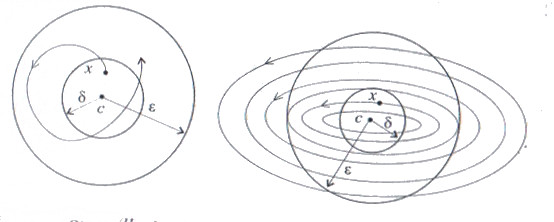
\includegraphics[scale=.5]{imagenes/circulo.jpg}
\end{center}

  


\begin{definicion}[Inestabilidad en puntos de equilibrio] 
	      Un punto de equilibrio $c$ se dice \emph{inestable} si no es estable.
 \end{definicion}            

\begin{ejercicio} Un punto de equilibrio $c$ es inestable si y sólo si existe
               un $\epsilon>0$,  una sucesión  de puntos $\{x_n\}$ y de tiempos $\{t_n\}$ tal que $t_n\in [0,b_{x_n})$, 
		$x_n\to c$ y $|\Phi_{t_n}(x_n)-c|\geq \epsilon$.
	    
\end{ejercicio}



 \noindent\emph{Observación.} Si $c$  es un punto de equilibrio estable de $X:\mathcal{O}\to\rr^n$ entonces $b_x=+\infty$.
 
Esta afirmación necesita una demostración. Tomemos $\epsilon>0$ tal que $\overline{B}(c,\epsilon)\subset\oo$. 
Por definición de estabilidad, existe $\delta>0$ tal que si $|x-c|<\delta$ y $t\in[0,b_x)$ entonces
$\Phi_t(x)\in B(c,\epsilon)$. Luego la imagen por la solución del intervalo $[0,b_x)$ está contenido dentro
de un compacto. Esto implica que $b_x=\infty$. 
 

\begin{definicion}[Estabilidad asintótica]
 {Definición: estabilidad asintótica} Un punto de equilibrio $c\in\oo$ se dice 
  \emph{asintóticamente estable} si es estable y existe $\delta>0$ tal que
  \[x\in B(c,\delta)\Rightarrow \lim_{t\to\infty}\Phi_t(x)=0.\]
  \end{definicion}  
 

 
 \subsection{Estabilidad via linealización}
 

\begin{teorema}[Estabilidad asintótica de sistemas lineales]
 Consideremos el sistema lineal $x'=Ax$, $A\in\rr^{n\times n}$.  Son equivalentes
  \begin{enumerate}
   \item El sistema lineal $x'=Ax$, $A\in\rr^{n\times n}$, tiene un equilibrio asintóticamente estable en $0$.
   \item Todo autovalor $\lambda$  de $A$ satisface que $\lambda\in (-\infty,0)$.
  \end{enumerate}
 
\end{teorema}

 

 


 \begin{teorema}[Invariancia de la estabilidad por equivalencias topológicas] Sean $X:\oo\to\rr^n$ e 
  $Y:\oo'\to\rr^n$ dos campos $C^1$ topológicamente equivalentes. Sea $f:\oo\to\oo'$ un homeomorfismo 
  que realiza esta equivalencia topológica entre $X$ e $Y$. Sea $c\in\oo$ un punto de equilibrio de $X$, recordar que
  $b:=f(c)$ lo es de $Y$. Entonces tenemos que  $c$ es (asintóticamente) estable  si y sólo si $d$ es 
  (asintóticamente) estable.
\end{teorema}
\begin{proof}
 Seguir los siguientes pasos. Demostrar  como  \emph{ejercicio} que si $\Phi_t^X$ y $\Phi_t^Y$ son los flujos asociados
 a $X$ e $Y$ respectivamente, entonces para cada $y\in\oo'$ y $t\in I_y$ vale que:
 \[\Phi_t^Y=f\circ\Phi_t^X\circ f^{-1}.\]
 Suponer $c$ estable y tomar $\epsilon>0$. Como $f$ es continua, $f^{-1}(B(b,\epsilon))$ es abierto
 y de allí existe $\epsilon_0>0$ tal que $B(c,\epsilon_0)\subset f^{-1}( B(b,\epsilon))$. Como  $c$ es estable, existe 
 $\delta_0$ tal que $\Phi_t^X(B(c,\delta_0))\subset B(c,\epsilon_0)$. Como $f^{-1}$ es continua, 
 $f(B(c,\delta_0))$ es abierto, luego existe $\delta>0$ tal que $B(b,\delta)\subset f(B(c,\delta_0))$. 
 Por todos los hechos previos,
 \[
  \begin{split} 
    \Phi_t^Y(B(b,\delta) )&=f\circ\Phi_t^X\circ f^{-1}(B(b,\delta) )\subset  f\circ\Phi_t^X(B(c,\delta_0))\\
	&\subset f(B(c,\epsilon_0)) \subset B(b,\epsilon).
   \end{split} 
 \]

 La afirmación recíproca, si $b$ es estable entonces $c$ lo es, sería redundante demostrarla. 
Para la estabilidad asintótica, supongamos $c$ asintóticamente estable y $\delta_0>0$  tal que 
\[x\in B(c,\delta_0)\Rightarrow \lim_{t\to\infty}\Phi_t^X(x)=0.\]
Por la continuidad de $f^{-1}$ existe $\delta>0$ tal que $B(b,\delta)\subset f(B(c,\delta_0))$. Luego, 
de estos hechos, el ejercicio previo, la continuidad de $f$ y $\Phi_t^X$ tenemos
que si $y\in B(b,\delta)$ entonces
 
 \[\lim_{t\to\infty}\Phi_t^Y(y)=\lim_{t\to\infty}f\circ\Phi_t^X\circ f^{-1}(y)=
 f\left( \lim_{t\to\infty}\Phi_t^X (f^{-1}(y))\right)=0\]
 
\end{proof}

\begin{corolario}
Supongamos que $c$ es un punto de equilibrio de $X:\oo\to\rr^n$. Supongamos que todos las partes reales de
 autovalores de 
 $DX(c)$ son negativas. Entonces $c$ es asintóticamente estable. Si en cambio, algún autovalor tiene parte real
 positiva, $c$ es inestable.
\end{corolario}

 El Corolario no afirma nada cuando hay autovalores imaginarios puros. Desafortunadamente esta situación se presenta con frecuencia.
Ejemplo de esto es la ecuación del resorte.
 


\subsection{Método de Lyapunov}

El método de Lyapunov está basado en la introducción de ciertas funciones, campos escalares 
 $\Lambda:U\to \rr$ donde $U$ es entorno de $c$. Estas funciones se llaman \href{http://es.wikipedia.org/wiki/Función_de_Lyapunov}{funciones de Lyapunov} y
 cumplen un papel análogo al de energía en sistemas mecánicos.
 
 A pesar del nombre, el método de Lyapunov no es del todo metódico, no tenemos un algorítmo para determinar 
 cuando existe una función de Lyapunov ni tampoco como puede ser obtenida.


\begin{definicion}[\href{http://es.wikipedia.org/wiki/Derivada_covariante}{derivada covariante}]
               Sea $X:\oo\to\rr^n$ un campo vectorial sobre el abierto $\oo\subset\rr^n$. La 
               \href{http://es.wikipedia.org/wiki/Derivada_covariante}{derivada covariante} respecto a $X$
               se simboliza por $\nabla_X$ y es un operador (difrencial) que actua sobre campos escalares 
               $F:\oo\to\rr$. Se define por
               \[
               \nabla_XF(x)=X\cdot\nabla F=\sum_{j=1}^nX_j(x) \frac{\partial F}{\partial x_j}(x).
                \]

\end{definicion}




\begin{ejercicio} Demostrar que
  \begin{enumerate}
    \item La derivada covariante de $F$ representa la variación de $F$ a lo largo de una 
   trayectoria del flujo asociado a $X$. En otros términos
   \[(\nabla_XF)(\Phi_t^X(x))=\frac{d}{dt}\left(F(\Phi_t^X(x)\right).\]
    \item $(\nabla_XF)(x)=|\nabla F(x)||X(x)|cos(\theta(x))$, donde $\theta(x)$ representa el ángulo entre $X(x)$ 
   y uno de los vectores normales a la superfice de la forma $\{y:F(y)=k\}$ que pasa por $x$.
  \end{enumerate}
\end{ejercicio}


\begin{definicion}[\href{http://es.wikipedia.org/wiki/Función_de_Lyapunov}{Función de Lyapunov}]
               Sea $X:\oo\to\rr^n$ un campo vectorial sobre el abierto $\oo\subset\rr^n$ y $c$ un punto de equilibrio.
               Una función, de clase $C^1$, $\Lambda:U\to\rr$, donde $U\subset\oo$ es  abierto y $c\in U$, se denomina
               \href{http://es.wikipedia.org/wiki/Función_de_Lyapunov}{Función de Lyapunov} para $c$ si satisface
               \begin{enumerate}
                 \item $\Lambda(c)<\Lambda(x)$ para todo $x\in U\setminus\{c\}$.
                 \item $\nabla_X\Lambda\leq 0$ en $U$.
                 \item Si se satisface la desigualdad estricta $\nabla_X\Lambda< 0$ diremos que $\Lambda$ es una 
                función de Lyapunov estricta.
               \end{enumerate}
\end{definicion}

              
  Acorde al inciso 2 de nuestro ejercico, la condición $(\nabla_X\Lambda)(x)\leq 0$ dice que el ángulo entre $X(x)$ 
 y la superficie  de nivel $\{z:\Lambda(z)=k\}$ que contiene al $x$ es obtuso ($(\nabla_X\Lambda)(x)<0$ ) 
 o, a lo sumo, recto ($(\nabla_X\Lambda)(x)=0$). 
 
   \begin{center}
   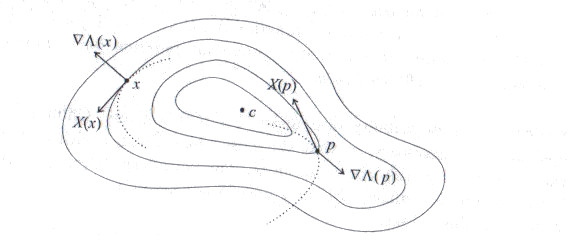
\includegraphics[scale=0.5]{imagenes/liapunov.jpg}
   \end{center}




  Visto a través del inciso 1) del ejercicio, una función de Liapunov satisface que tiene un mínimo en $c$ 
 y que $\Lambda(\Phi_t^X(x))$ es decreciente respecto al tiempo.  Esta observación es la idea clave para demostrar el Teorema de Estabilidad de Lyapunov.


\begin{teorema}[Teorema de Estabilidad  de Lyapunov]
  Sea $X:\oo\to\rr^n$ un campo vectorial sobre el abierto $\oo\subset\rr^n$ y $c$ un punto de equilibrio.
               Supongamos que $\Lambda:U\to\rr$, con $U\subset\oo$ abierto y $c\in U$, es una
               \href{http://es.wikipedia.org/wiki/Función_de_Lyapunov}{Función de Lyapunov} para $c$. Entonces $c$ 
               es un equilibrio estable. Si $\Lambda$ es una función de Lyapunov estricta para $c$, entonces $c$ es 
               asintóticamente estable.
 \end{teorema}

\begin{proof}  Sea $\epsilon>0$. Tomemos $0<\epsilon_0$ tal que $\epsilon_0\leq\epsilon$ y 
$\overline{B}(c,\epsilon_0)\subset U$.  Como $\partial B(c,\epsilon_0)$ es un compacto y $\Lambda$ es continua, $\Lambda$
alcanza un valor mínimo sobre aquel conjunto, es decir existe $z_0$, con $|z_0-c|=\epsilon_0$ tal que
\begin{equation}\label{minimo}
 \mu:=\min\{\Lambda(y):|y-c|=\epsilon_0\}=\Lambda(z_0)>\Lambda(c).
\end{equation}

 Sea ahora $\delta>0$ tal que 
\[B(c,\delta)\subset B(c,\epsilon_0)\cap \Lambda^{-1}(-\infty,\mu).\]
ver figura \ref{dem_lya}.



 {Teorema de Estabilidad  de Lyapunov}
  \begin{figure}[h]
    \begin{center}
   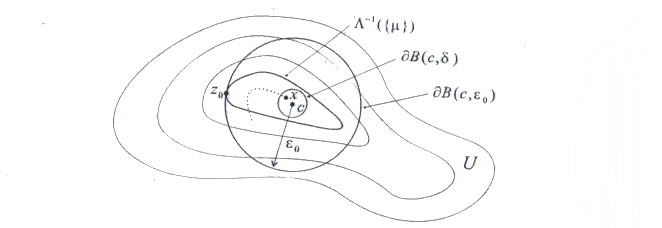
\includegraphics[scale=0.5]{imagenes/dem_lya.jpg}
   \caption{Demostración Teorema Lyapunov}\label{dem_lya}
   \end{center}
 \end{figure}


{Teorema de Estabilidad  de Lyapunov}
  Supongamos ahora que $x\in B(c,\delta)$. Como $\Lambda(x)<\mu$ y como $\Lambda\left(\Phi_t(x)\right)$ es decreciente para 
 $t\in [0,b_x)$ tenemos que 
 \begin{equation}\label{decrec}
  \Lambda(\Phi_t(x))<\mu\quad\hbox{para } t\in [0,b_x).
 \end{equation}

 Vemos que $\Phi_t(x)\in B(c,\epsilon_0)$ cuando $t\in [0,b_x)$. De lo contrario existiría un $t_0>0$ con 
$\Phi_{t_0}(x)\notin B(c,\epsilon_0)$. Como $\Phi_t(x)$ es continua respecto a $t$, el conjunto 
$\{\Phi_t(x)|t\in[0,t_0]\}$ es conexo. Por consiguiente 
$ \{\Phi_t(x)|t\in[0,t_0]\}\cap \partial B(c,\epsilon_0)\neq\emptyset$. Luego existiría un $t\in[0,t_0]$ tal que
$\Phi_{t_0}(x)\in \partial B(c,\epsilon_0)$. Para este $t_0$ por \eqref{minimo} tendremos que 
$\Lambda(\Phi_{t_0}(x))\geq \mu$ que contradice \eqref{decrec}. Como $B(c,\epsilon_0)\subset B(c,\epsilon)$, hemos
demostrado la estabilidad. 

 
Supongamos la función de Lyapunov $\Lambda$ estricta. Veamos que si $x\in B(c,\delta)$ entonces 
$\Phi_t(x)\to c$ cuando $t\to\infty$. De no ser esto último cierto, existiría un 
$\epsilon_1>0$ y una sucesión de tiempos $t_k$ tendiente a $+\infty$ tal que
\[
 |\Phi_{t_k}(x)-c|\geq \epsilon_1.
\]
Como $\Phi_{t_k}(x)\in \overline{B}(c,\epsilon_0)$ y este conjunto es compacto, existiría una subsucesión de $\Phi_{t_k}(x)$
convergente. Por simplicidad supondremos que esta subsucesión es $t_k$ y llamaremos $z$ a este límite. 

 
 
Ahora $\Lambda(\Phi_t(z))$ es decreciente respecto a $t$, por ello existe $s>0$ tal que $\Lambda(\Phi_s(z))<\Lambda(z)$. Como
la función $y \mapsto \Lambda(\Phi_s(y))$ es continua en $y$ para $s$ fijo, existe un entorno $V$ de $z$ tal que si 
$y\in V$ entonces $\Lambda(\Phi_s(y))<\Lambda(z)$. Como  $\Phi_{t_k}(x)$ tiende a $z$, existiría $K>0$ tal que 
$\Phi_{t_k}(x)\in V$, cuando $k>K$. Fijemos uno de tales $k$, lo llamaremos $k_0$. Ahora si elegimos cualquier $k$
suficientemente grande para que $t_k>t_{k_0}+s$, tendremos
\[\Lambda(z)\leq \Lambda(\Phi_{t_k})<\Lambda(\Phi_{t_{k_0}+s})=\Lambda(\Phi_s(\Phi_{t_{k_0}}(x)))<\Lambda(z).\]


\end{proof}




\subsection{Método de Lyapunov: Ejemplos}

\begin{ejemplo} Estabilidad de los equilibrios $2k\pi$, $k\in\mathbb{Z}$, en la ecuación del péndulo

\end{ejemplo}
 \begin{sageblock}
x,y=var('x,y')
Eq1=y
Eq2=-sin(x)
Equilibrios=solve([Eq1,Eq2],[x,y])
Equilibrios
\end{sageblock}
Sagemath encuentra los equilibrios $\sage{Equilibrios}$, que es su manera de expresar $x=n\pi$, $y=0$, con $n\in\mathbb{Z}$. Analicemos el equilibrio $(0,0)$. 

\begin{sageblock}
X(x,y)=[Eq1,Eq2]
A=X.diff()(0,0)
D=A.eigenmatrix_right()
\end{sageblock}

\[\sage{D}\]
No  se puedo aplicar el Teorema Linearización, autovalores imaginarios puros. Vamos a usar la energía

\[E=\frac{1}{2}y^2-\cos(x)\]

como función de Lyapunov.
\begin{sageblock}
Lambda(x,y)=1/2*y^2-cos(x)
p=plot3d(Lambda,(x,-5,5),(y,-1,1))
\end{sageblock}
\begin{center}
\sageplot[][png]{plot3d(Lambda,(x,-5,5),(y,-1,1))}
\end{center}
Es facil demostrar que 
\[\Lambda(x,y)>\Lambda(0,0)\quad\hbox{para } -2\pi<x<\pi,\,\, y\in\mathbb{R},(x,y)\neq(0,0)\]
Calculamos la derivada covariante.

\begin{sageblock}
DLambdaX=Lambda.diff().dot_product(X)
\end{sageblock}

\[\sage{DLambdaX}\]

Como es no positiva, $\Lambda$ es una función de Lyapunov y por consiguiente $(0,0)$ es estable. Es interesante analizar las curvas de nivel de la función de Lyapunov.
\begin{sageblock}
p=contour_plot(Lambda,(x,-2*pi,2*pi),(y,-3,3),contours=srange(-1,5,.2),fill=False)
\end{sageblock}

\begin{center}
\sageplot[width=.9\linewidth][png]{p}
\end{center}

\begin{ejemplo}\emph{\cite[ Ejemplo 6.1 ]{DavidBetounes488}}
\[X(x,y,z)=(y(z-1),x(z+1),-2xy)\]
\begin{sageblock}
x,y,z=var('x,y,z')
Eq1=y*(z-1)
Eq2=x*(z+1)
Eq3=-2*x*y
Equilibrios=solve([Eq1,Eq2,Eq3],[x,y,z])
\end{sageblock}
Encontramos los equilibrios
\[\sage{Equilibrios}\]
Vamos a analizar el $(0,0,0)$ Estamos en problemas para aplicar el Teorema de Linearización, ni siquiera los puntos de equilibrio estan aislados. Un teorema afirma que equilibrio hiperbólico está aislado de otros equilibrios.
\begin{sageblock}
X(x,y,z)=[Eq1,Eq2,Eq3]
A=X.diff()(0,0,0)
D=A.eigenmatrix_right()
\end{sageblock}
\[D=\sage{D}\]
Como adelantamos, la linearización no es posible. Vamos a demostrar que
\[\Lambda(x,y,z)=\frac12(x^2+y^2+z^2),\]
es una función de Lyapunov para el equilibrio $(0,0,0)$. Claramente $\Lambda$ tiene un mínimo en $(0,0,0)$. 
\begin{sageblock}
Lambda(x,y,z)=1/2*(x^2+y^2+z^2)
DX=Lambda.diff().dot_product(X).simplify_full()
\end{sageblock}
\[DX=\sage{DX}.\]
Por el Teorema de Lyapunov $(0,0,0)$ es estable. Grafiquemos las superficies de nivel y algunas soluciones.
\begin{sageblock}
def X(t,x):
    return [ x[1]*(x[2]-1),x[0]*(x[2]+1),-2*x[0]*x[1]]

T =  ode_solver()
T.function=X
T.algorithm="rk8pd"
A=[]
T.ode_solve(y_0=[1,1,1],t_span=[0,30], num_points=100)
a=T.solution
Sol=[soln[1] for soln in a]
Gra=list_plot(Sol,plotjoined=True,thickness=.5,rgbcolor=(1,0,0))
theta,phi=var('theta,phi')
Esfe=parametric_plot3d([sqrt(3.0)*cos(theta)*sin(phi), sqrt(3.0)*sin(theta)*sin(phi), sqrt(3.0)*cos(phi)], (theta,0,2*pi), (phi,0,pi),opacity=0.4)
Gra+=Esfe
T.ode_solve(y_0=[1,0,sqrt(2)],t_span=[0,30], num_points=100)
a=T.solution
Sol=[soln[1] for soln in a]
Gra+=list_plot(Sol,plotjoined=True,thickness=.5,rgbcolor=(1,0,0))
T.ode_solve(y_0=[1,0,-sqrt(2)],t_span=[0,30], num_points=100)
a=T.solution
Sol=[soln[1] for soln in a]
Gra+=list_plot(Sol,plotjoined=True,thickness=.5,rgbcolor=(1,0,0))
T.ode_solve(y_0=[-1,0,-sqrt(2)],t_span=[0,30], num_points=100)
a=T.solution
Sol=[soln[1] for soln in a]
Gra+=list_plot(Sol,plotjoined=True,thickness=.5,rgbcolor=(1,0,0))
\end{sageblock}
\begin{center}
\sageplot[width=.9\linewidth][png]{Gra}
\end{center}



\end{ejemplo}



\section{Estabilidad d órbitas periódicas}

\subsection{Definiciones} 
 Recordemos: si $X:\oo\to\rr^n$ es un campo de clase $C^1$ y  $x\in\oo$, entonces $I_x=(a_x,b_x)$ denota el intervalo máximo
 de definición de la solución $\gamma$ que satisface que $\gamma(0)=x$

 \begin{definicion}[Estabilidad de Soluciones en General]
 Sea $X:\oo\to\rr^n$ es un campo de clase $C^1$ y  $c\in\oo$. Sea $\gamma:I_c\to\oo$ la solución tal que 
 $\gamma(0)=c$. Diremos que $\gamma$ es \emph{estable} si para cada $\epsilon>0$ existe $\delta>0$ con 
 $B(c,\delta)\subset\oo$ y si $x\in B(c,\delta)$ entonces:
 \begin{enumerate}
  \item $[0,b_c)\subset [0,b_x)$
  \item $|\Phi_t(x)-\gamma(t)|<\epsilon$, para todo $t\in[0,b_c)$. 
 \end{enumerate}
  Si además tenemos que $b_x=+\infty$ y
 \[\lim_{t\to\infty}|\Phi_t(x)-\gamma(t)|=0, \]
 diremos que $\gamma$ es \emph{asintóticamente estable}.
\end{definicion}


   \begin{center}
   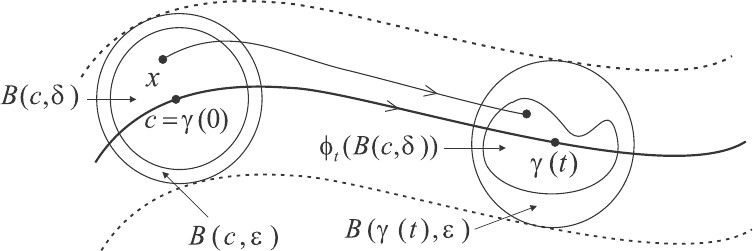
\includegraphics[scale=0.4]{imagenes/estabilidad_gral.jpg}
   \end{center}




\subsection{Ecuaciones Variacionales}

 Si desarrollamos en serie de Taylor $X$ alrededor de cualquier $x\in\oo$, tenemos para $h\in\rr^n$ chico
 \[X(x+h)=X(x)+DX(x)h+\cdots\]
Supongamos $\gamma$ la solución de la cual queremos considerar su estabilidad, y sea $\alpha$ otra solución 
(luego habrá que suponer que $\alpha(0)$ es cercano a $\gamma(0)$). Escribamos $\alpha=\gamma+\xi$. Se suele
decir que $\xi$ es la variación de $\gamma$. ¿Resolverá alguna ecuación $\xi$? Reemplazando en el desarrollo de Taylor
$x$ por $\gamma$ y $h$ por $\xi$ y desestimando los términos de mayor orden vemos $\xi$ resolvería aproximadamente

\[\xi'(t)=DX(\gamma(t))\xi(t).\]


$X:\oo\to\rr^n$ es un campo de clase $C^1$ y $\gamma:I\to\oo$ una solución. A la función a valores matriciales
$A(t)=DX(\gamma(t))$ la llamaremos \emph{matriz variacional} o \emph{matriz de \href{http://es.wikipedia.org/wiki/Monodromía}{monodromía}}. 

El sistema lineal asociado
$x'(t)=A(t)x(t)$ se llama el sistema de \emph{ecuaciones variacionales}. 
 
La matriz fundamental de este sistema 
$G:I\to\rr^{n\times n}$ se llama la \emph{matriz característica}. 

Sea $\gamma$ una solución periódica que no es un equilibrio. Entonces existe un período $p>0$ mínimo
entre todos los períodos positivos. Esto es $\gamma(x+p)=\gamma(x)$  y cualquier otro período es múltiplo de $p$. 
Es sabido que en este caso el dominio máximo de definición de $\gamma$ es $\rr$. En esta situación definiremos
los \emph{multiplicadores característicos} de $\gamma$ como los autovalores de $G(p)$.




\subsection{Ejemplos}

\begin{ejemplo}\emph{\cite[ Ejemplo 6.3 ]{DavidBetounes488}} Considerar el sistema
\[
\left\{
 \begin{array}{cc}
  x'&=-y+xz\\
  y'&=x+yz\\
  z'&=-z(x^2+y^2)\\
 \end{array}
\right.
\]
Vale decir $X:\mathbb{R}^3\to\mathbb{R}^3$, es el campo
\[X(x,y,z)=(-y+xz,x+yz,-z(x^2+y^2))\]
Computemos la matríz Jacobiana
\begin{sageblock}
x,y,z,t=var('x,y,z,t')
X(x,y,z)=(-y+x*z,x+y*z,-z*(x^2+y^2))
DX=X.diff()(x,y,z)
\end{sageblock}

\[
DX=\sage{DX}
\]
La función  $\gamma(t)=(\cos(t),\sin(t),0)$ es solución de periódica de periodo $2\pi$. Computemos la matríz de monodromía.
\begin{sageblock}
A=(X.diff())(cos(t),sin(t),0).simplify_trig()
\end{sageblock}
\[A=\sage{A}.\]
 Las ecuaciones características
 \begin{sageblock}
Eq=A*vector([x,y,z]).column()
\end{sageblock}
\[Eq=\sage{Eq}.\]

Para resolverlas notar que la tercera ecuación está desacoplada de las dos primeras.  SAGE no sabe sacar provecho de eso. Lo tenemos que ayudar un poco
\begin{sageblock}
t=var('t')
x=function('x',t)
y=function('y',t)
z=function('z',t)
z_sol=desolve( z.diff(t)==-z,z)
\end{sageblock}
\[z=\sage{z_sol}.\]
\begin{sageblock}
a,b,c=var('a,b,c')
Sol=desolve_system([x.diff(t)==c*e^(-t)*cos(t)-y\
    ,y.diff(t)==sin(t)*c*e^(-t)+x],[x,y],ivar=t,ics=[0,a,b])
\end{sageblock}
\[
 \begin{array}{l}
  \sage{Sol[0]}\\
  \sage{Sol[1]}
 \end{array}
\]
Calculamos la matriz fundamental del sistema, que resulta ser la matríz característica de $\gamma$.
\begin{sageblock}
c1=Sol[0].rhs()
c2=Sol[1].rhs()
c3=c*exp(-t)
e1={a:1,b:0,c:0}
e2={a:0,b:1,c:0}
e3={a:0,b:0,c:1}
G=matrix([\
[c1.substitute(e1),c1.substitute(e2),c1.substitute(e3)]\
,[c2.substitute(e1),c2.substitute(e2),c2.substitute(e3)]\
,[c3.substitute(e1),c3.substitute(e2),c3.substitute(e3)]])

\end{sageblock}
\[G=\sage{G}.\]
Por último los multiplicadores característicos

\begin{sageblock}
D=G.subs(t=2*pi).eigenmatrix_right()
\end{sageblock}
\[\sage{D}\]
\end{ejemplo}

 \begin{ejemplo}\emph{\cite[ Ejemplo 6.4 ]{DavidBetounes488}} Hallar matriz de mondrom´ia y multiplicadores caracter´isiticos para el sistema 2-dimensional
 \[
 \begin{array}{cc}
  x'(t)&=-x-b*y+x^3+x*y^2\\
  y'(t)&=b*x-y+x^2*y+y^3
 \end{array}
 \]

\begin{sageblock}
x,y,t,b=var('x,y,t,b')
X(x,y)=(-x-b*y+x^3+x*y^2,b*x-y+x^2*y+y^3)
\end{sageblock}   

Si se expresa el sistema en coordenandas polares se puede demostrar que $\gamma(t)=(\cos(b*t),\sin(b*t))$ es solución periódica de período $2\pi/b$. Chequeemos esta última afirmación de manera directa.
\begin{sageblock}
((X(cos(b*t),sin(b*t)))[0]-(cos(b*t)).diff(t)).simplify_full()
((X(cos(b*t),sin(b*t)))[1]-(sin(b*t)).diff(t)).simplify_full()
\end{sageblock} 
Matríz de Monodromía
\begin{sageblock}
A(t)=(X.diff())(cos(b*t),sin(b*t)).simplify_trig()
\end{sageblock} 
\[A(t)=\sage{A(t)}.\]
\begin{ejercicio}
 Demostrar que la matríz característica viene dada por: 
 \begin{sageblock}
 G=matrix([[e^(2*t)*cos(b*t)  , -sin(b*t) ]\
 ,[e^(2*t)*sin(b*t)  , cos(b*t) ]])
 \end{sageblock} 
 \[G=\sage{G}.\]

\end{ejercicio}
 Multiplicadores característicos
  \begin{sageblock}
D=G.subs(t==2*pi/b).eigenmatrix_right()
 \end{sageblock} 
  \[D=\sage{D}.\]


 \end{ejemplo}






\subsection{Matriz de deformaciones} 

\begin{definicion}Supongamos
  $X:\oo\to\rr^n$ es un campo de clase $C^1$ y $\Phi_t:\mathcal{D}\subset\rr\times\rr^n\to\oo$ el flujo asociado. 
 Definimos la \emph{matriz de deformaciones} $H$ como 
 \[H(t,x)=(D_x\Phi_t)(x)=\begin{pmatrix}
                        \frac{\partial\Phi^1_t}{\partial x_1 } &\dots & \frac{\partial\Phi^1_t}{\partial x_n}\\
                        \vdots  & \ddots & \vdots\\
                        \frac{\partial\Phi^n_t}{\partial x_1 }& \dots &\frac{\partial\Phi^n_t}{\partial x_n }\\ 
                       \end{pmatrix}
\]
\end{definicion}






 

\begin{teorema}Sea $\gamma:I\to\oo$ una solución, con $0\in I$ y $c=\gamma(0)$. La matriz característica 
$G$ de $\gamma$ coincide con la matriz de deformaciones $H$ en $c$:
\[G(t)=H(t,c).\]
Además
\[G(t)X(c)=X(\gamma(t))\quad t\in I.\]
Luego si $\gamma$ es periódica de período $p$ tenemos
\[G(p)X(c)=X(c).\]
Entonces $1$ es un autovalor y $X(c)$ (como $\gamma$ no es equilibrio $X(c)\neq 0$) es un autovector asociado.
En conclusión $1$ es siempre un multiplicador característico.
 
\end{teorema}



\begin{proof}
 Derivando respecto a $x$ la relación

\[\frac{d}{dt}\Phi_t(x)=X(\Phi_t(x)),\]
Obtenemos
\[\frac{\partial H}{\partial t}(t,x)=D_xX(\Phi_t(x))H(t,x)\]
Además $H(0,x)=I$, donde $I$ es la identidad (\textbf{Ejercicio}). Como $\gamma(t)=\Phi_t(c)$ si reemplazamos $x$
por $c$ arriba tenemos 
\[
 \frac{\partial H}{\partial t}(t,c)=A(t)H(t,c)
\]
Lo cual termina por mostrar que $G(t)=H(t,c)$. 


 Ahora derivando
 \[\gamma'(t)=X(\gamma(t)),\]
 vemos que
  \[\gamma''(t)=D_xX(\gamma(t))\gamma'(t)=A(t)\gamma'(t),\]
  es decir que $\gamma'(t)$ es solución de las ecuaciones características. Además $\gamma'(0)=X(\gamma(0))=X(c)$. 
  Ahora como $G$ es una matriz fundamental para las ecuaciones características
  \[X(\gamma(t))=\gamma'(t)=G(t)X(c).\]
  Esto prueba la segunda afirmación. La tercera es consecuencia de que $\gamma(p)=\gamma(0)=c$.
\end{proof}


 
 

 \begin{teorema}



Sea $f:\oo\to\tilde{\oo}$ un difeomorfismo entre abiertos de $\rr^n$, $X:\oo\to\rr^n$ un campo $C^1$ e $Y:\tilde{\oo}\to\rr^n$ su push-forward, es decir $Y=f_*(X)$.
Sean $H^X$ y $H^Y$ las matrices de deformaciones de los campos $X$ e $Y$ respectivamente. Tambien consideramos los flujos $\Phi_t^X$ y $\Phi_t^Y$. Se tiene la siguiente 
relación
\begin{equation}\label{def_mat}H(t,y)=Df(\Phi^X_t(f^{-1}(y)))H(t,f^{-1}(y)) \left(Df(f^{-1}(y))\right)^{-1}.\end{equation}


Si $\gamma:I\to\oo$ es una solución de $x'=X(x)$, entonces $\beta=f\circ\gamma$ es solución de $y'=Y(y)$. Las matrices características 
de $\gamma$ y $\beta$, digamos  $G^X$ y $G^Y$ respectivamente, son similares. Especificamente
\begin{equation}\label{car_mat}G^Y(t)=D_xf(\gamma(t))G^X(t)\left(D_xf(c)\right)^{-1}.\end{equation}
En particular si $\gamma$ es periódica de periodo $p$, $\beta$ es periódica con el mismo periodo y los multiplicadores característicos son los mismos.

 \end{teorema}


 
\begin{proof}
 Derivando respecto a $y$ la siguiente relación, que es sabido que ocurre,
\[\Phi_t^Y(y)=(f\circ \Phi^X_t\circ f^{-1})(y),\]
y usando la regla de la cadena obtenemos \eqref{def_mat}. Supongamos que $\gamma(0)=c$. Entonces $\gamma(t)=\Phi^X_t(c)$, $\beta(0)=f(c)$ y $\beta(t)=\Phi_t^Y(f(c))$. 
Luego, reemplazando $y$ por $f(c)$ en \eqref{def_mat} llegamos a  \eqref{car_mat}.  Reemplazando en esta última ecuación $t$ por el período $p$ vemos que $G^Y(p)$ y $G^X(p)$
son similares, de allí tienen el mismo espectro.\end{proof}
 
 
 \subsection{Radio espectral}

\begin{definicion}[Radio espectral] Sea $A\in\rr^{n\times n}$ una matriz, definimos su
\href{http://es.wikipedia.org/wiki/Radio_espectral}{radio espectral} $\rho(A)$ por
\[
\rho(A):= \sup\{|\lambda|: \lambda\in\sigma(A)\}.
\]
Aquí, como es usual, $\sigma(A)$ es el espectro de $A$.

 \end{definicion}




Sea $\mathcal{F}$ la familia de todas las normas sobre $\rr^n$. Si $A\in\rr^{n\times n}$ y $\|\cdot \|\in\mathcal{F}$, 
por abuso de notación seguiremos usando el mismo símbolo $\|A\|$ para la norma como operador sobre $A$ inducida por 
$\|\cdot\|$. Es decir
\[\|A\|:=\sup_{\|x\|\leq 1} \|Ax\|\]


\begin{teorema}[Una representación del radio espectral]



  Sea $A\in\rr^{n\times n}$. Entonces
\[  \rho(A)=\inf_{\|\cdots\|\in\mathcal{F}}\|A \|. \]

\end{teorema}

\begin{corolario}





\begin{enumerate}
 \item Sea $A\in\rr^{n\times n}$ y $\epsilon>0$. Entonces existe una norma $\| \cdot\|\in\mathcal{F}$ tal que
\[  \rho(A)\leq \|A\|<\rho(A)+\epsilon.\]
\item Si $\rho(A)<1$ existirá una norma $\|\cdot\|_0$, para la cual $A$ es una contracción, es decir $\|Ax\|_0<q\|x\|_0$ y $q<1$. 

\item Si $\rho(A)<1$ entonces $A^kx\to 0$ cuando $k\to\infty$.
\end{enumerate}

\end{corolario}

 

\subsection{Discución heurística}
Sea $\gamma(t)$ una solución periódica de período $p$ con $\gamma(0)=c$ y $X(c)\neq 0$. Sea $\mu_1,\mu_2,\dots,\mu_n$ los autovalores de $G(p)$, 
es decir los
multiplicadores característicos de $\gamma$. Como $1$ es autovalor, podemos suponer $\mu_1=1$. Un autovector asociado es $X(c)$. Sea $M_c$ el hiperplano ortogonal a $X(c)$
que contiene a $c$, $M_c=\{x|(x-c)\cdot X(c)=0\}$. 

Vamos a demostrar  que si $|\mu_j|<1$, $j=2,\ldots,n$ entonces $G(p)$ restrigida a $M_c$ es una contracción.

Consideremos $\alpha$ una solución cercana en $t=0$ a $\gamma$. Como vimos podemos escribir 
\begin{equation}\label{ecuaaprox}
 \alpha\approx \gamma+\xi,
\end{equation}
 donde $\xi$ resuelve las ecuaciones 
variacionales $\xi'(t)=A(t)\xi(t)$. Como $G(t)$ es una matriz fundamental para ese sistema 
\begin{equation}\label{ecuavar}
 \xi(t)=G(t)\xi(0). 
\end{equation}





\begin{ejercicio}
 Demostrar que si $A(t)$ es una función a valores matriciales $A:I\subset\rr\to\rr^{n\times n}$ que además es periódica con periodo $p$,
entonces la matriz fundamental satisface que $G(t+p)=G(t)G(p)$. En particular
\begin{equation}\label{semigrupo}G(kp)=G(p)^k.\end{equation}
Considerando los tiempos $t=p,2p,\ldots$ y usando \eqref{ecuaaprox}, \eqref{ecuavar} y \eqref{semigrupo} llegamos a
\[\alpha(kp)=c+G(p)^k\xi(0),\]
\end{ejercicio}


Vamos a ver que todo solución cercana a $\gamma$ atraviesa $M_c$, así podremos suponer que $\xi(0)\in M_c$. Luego si $|\mu_j|<1$, $j=2,\ldots,n$, 
entonces $\alpha(kp)\to c$. 

Esta discusión da un indicio de por que podremos esperar estabilidad si  $|\mu_j|<1$, $j=2,\ldots,n$.






\subsection{Estabilidad orbital}
\begin{definicion}[Estabilidad orbital]
  Sea $\gamma$ una solución periódica y $\Gamma=\gamma(\rr)$. Diremos que $\gamma$ es \emph{orbitalmente estable} si para cada $\epsilon>0$ existe $\delta>0$ tal que
 \[d(x,\Gamma)<\delta\Rightarrow d(\Phi_t(x),\Gamma)<\epsilon.\]
 Si además tenemos que
  \[\lim_{t\to +\infty}d(\Phi_t(x),\Gamma)=0,\]
  diremos que $\gamma$ es \emph{orbitalmente asintóticamente estable}
\end{definicion}




\subsection{Mapeo de Poincaré}


\begin{teorema}[Mapeo de Poincaré]
 Sea $\gamma:\rr\to\oo$ una solución de período $p$ del sistema $x'=X(x)$, donde $X:\oo\to \rr^n$. Sea $c$ y $M_c$ como antes. Entonces existe un entorno abierto $U$ de $c$ 
 y una función $C^1$ $\tau:U\to \rr$ tal que $\tau(c)=p$
 \[\Phi_{\tau(x)}\in M_c\]
La aplicación $P:U\cap M_c\to M_c$ dada por $P(x)=\Phi_{\tau(x)}(x)$ se llama \href{http://es.wikipedia.org/wiki/Aplicación_de_Poincaré}{Mapeo de Poincaré}.
\end{teorema}

\begin{proof} Definimos
\[F(t,x)=(\Phi_t(x)-c)\cdot X(x).\]
Se tiene que $F(p,c)=0$ y que
\[\frac{\partial}{\partial t}F(t,x)=X(\Phi_t(x))\cdot X(x).\]
Luego
\[\frac{\partial F}{\partial t}(p,c)=|X(c)|^2>0.\]


Se satisfacen las hipótesis del teorema de la función implícita, por consiguiente existe un entorno abierto $V$ de $(p,c)$  y un entorno $U$ de $c$ tal que
\[\{(t,x)\in V|F(t,x)=0\}=\{(t,x)|x\in U\hbox{ y }t=\tau(x)\}\]
Vale decir $F(\tau(x),x)=0$, lo que implica $\Phi_{\tau(x)}(x)\in M_c$\qed


 
   \begin{center}
   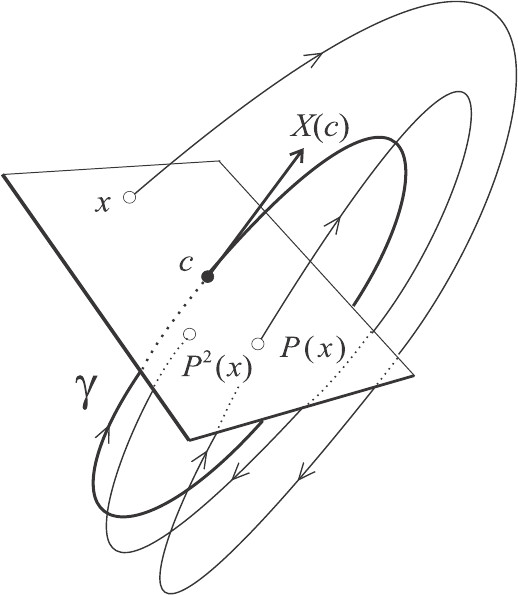
\includegraphics[scale=0.3]{imagenes/poincaremap.jpg}
   \end{center}


\begin{ejemplo} Hallar el Mapeo Poincaré de

 \[\begin{cases} x'(t)&= x\left(t\right)^{3} + x\left(t\right)
y\left(t\right)^{2} - b y\left(t\right) - x\left(t\right)\\
y'(t) &= x\left(t\right)^{2} y\left(t\right) +
y\left(t\right)^{3} + b x\left(t\right) - y\left(t\right)\\   
  \end{cases}\]


Convirtiendo a polares
\[
 \begin{cases}
  r'(t)&=r(t)(r^2(t)-r(t))\\
  \theta'(t)&=b.
 \end{cases}
\]
ver \href{http://sage.ccad.unrc.edu.ar/home/pub/63/}{Sigue en notebook de SAGE}


{Producto tensorial}
Dados dos vectores $a,b\in\mathbb{R}^n$ definimos su producto tensorial $a\otimes b$ como el operador lineal  $a\otimes b:\rr^n\to\rr^n$ definido por
\[\left(a\otimes b\right)v=\left(b\cdot v\right)a,\quad \text{ para } v\in\rr^n.\]
\textbf{Ejercicio} Demostrar que respecto a la base canónica de  $\rr^n$ la representación matricial del operador $a\otimes b$ tiene entrada $ij$
\[\left(a\otimes b\right)_{ij}=a_ib_j.\]

El mapeo de Poincaré $P$ está definido en $U\cap M_c$, pero podemos extenderlo $\tilde{P}:U\to\rr^n$ por
\[\tilde{P}(x)=\Phi_{\tau(x)}(x).\]




{Matriz Jacobiana Mapeo Poincaré}
\textbf{Ejercicio:} Demostrar que
\[D\tilde{P}(x)=X(\tilde{P}(x))\otimes\nabla\tau(x)+H(\tau(x),x),\]
en particular
\[D\tilde{P}(c)=X(c)\otimes\nabla\tau(c)+G(p).\]



{Matriz Jacobiana Mapeo Poincaré}
{Teorema Matriz Jacobiana Mapeo Poincaré}
 Asumamos $c=0$ y $X(0)=(0,0,\ldots,0,1)$. Entonces:
 \begin{equation}\label{gp}G(p)=\begin{bmatrix}
         b_{11}&\cdots&b_{1,n-1}&0\\
        \vdots &\ddots&\vdots&0\\
         b_{n-1,1}&\cdots&b_{n-1,n-1}&0\\
         *&\cdots&*&1\\
        \end{bmatrix}
 \end{equation}
 
 \begin{equation}\label{dptil}D\tilde{P}(0)=\begin{bmatrix}
         b_{11}&\cdots&b_{1,n-1}&0\\
        \vdots &\ddots&\vdots&0\\
         b_{n-1,1}&\cdots&b_{n-1,n-1}&0\\
         *&\cdots&*&*\\
        \end{bmatrix}
\end{equation}






{Matriz Jacobiana Mapeo Poincaré}
{Matriz Jacobiana Mapeo Poincaré}
Al subespacio $M_0=\{(x_1,\ldots,x_{n-1},0)|x_i\in\rr\}$ lo identificamos con $\rr^{n-1}$ y al abierto relativo $U\cap M_0$ con un abierto $V$ de $\rr^{n-1}$. 
Con estas identificaciones podemos pensar en el Jacobiano de $P:V\to \rr^{n-1}$ siendo este en $c=0$ dado por
 \begin{equation}\label{dp}DP(0)=\begin{bmatrix}
         b_{11}&\cdots&b_{1,n-1}\\
        \vdots &\ddots&\vdots\\
         b_{n-1,1}&\cdots&b_{n-1,n-1}\\
        \end{bmatrix}
\end{equation}
Luego si $\mu_1=1,\mu_2,\ldots,\mu_n$ son los multiplicadores característcos de $\gamma$ entonces $\mu_2,\ldots,\mu_n$ son autovalores de $DP(0)$.







{Matriz Jacobiana Mapeo Poincaré}
\textbf{Demostración} Como $G(p)X(0)=X(0)$ y como $X(0)=(0,0,\ldots,0,1)$ vemos que la enésima columna de $G(p)$ es también el enésimo vector canónico. Esto justfica 
\eqref{gp}.
Tenemos que
\[
 X(0)\otimes\nabla\tau(0)=\begin{bmatrix}
         0&\cdots&0&0\\
        \vdots &\ddots&\vdots&0\\
         0&\cdots&0&0\\
         *&\cdots&*&*\\
        \end{bmatrix}
\]
Como $D\tilde{P}(0)=X(0)\otimes\nabla\tau(0)+G(p)$ se tiene \eqref{dptil}.



{Matriz Jacobiana Mapeo Poincaré}
Sea $I_k$ la matriz identidad de $k\times k$, $B$ la matriz $B=\{b_{ij}\}_{i,j=1}^{n-1}$. Como
\[\det (G(p)-\mu I_n)=(1-\mu)\det (B-\mu I_{n-1}),\]
los autovalores de $B$ son precisamente $\mu_2,\ldots,\mu_n$.

Consideramos la incrustación $i:\rr^{n-1}\to\rr^n$, dada por $i(x_1,\ldots,x_{n-1})=(x_1,\ldots,x_{n-1},0)$ y la proyección
 $\rho:\rr^{n}\to\rr^{n-1}$,  dada por $\rho(x_1,\ldots,x_{n})=(x_1,\ldots,x_{n-1})$. Con esta notación
 \[P(v)=\rho(\tilde{P}(i(v))),\quad\text{ para } v\in V=\rho(U\cap M_0)\]
 por la regla de la cadena,
 \[DP(0)=\begin{bmatrix}
         I_{n-1}&0_{(n-1)\times n}\\
        \end{bmatrix}
        \begin{bmatrix}
         B&0_{(n-1)\times n}\\
         *&*\\
        \end{bmatrix}
        \begin{bmatrix}
         I_{n-1}\\0_{n\times (n-1)}\\
        \end{bmatrix} =B
  \]
\qed


{Matriz Jacobiana Mapeo Poincaré}
\textbf{Ejercicio} ¿Cómo podemos reducir el caso general $c$ no necesariamente $0$ y $X(c)\neq 0$ al caso cosiderado? 



{Teorema Estabilidad Orbital}
{Teorema Estabilidad Orbital} 
 Sea $\gamma:\rr\to\oo$ una solución de período $p$ del sistema $x'=X(x)$, donde $X:\oo\to \rr^n$. Sea $c=\gamma(0)$ y $M_c$ como antes. Supongamos que $n-1$ de los múltiplos 
 característicos $\mu_2,\ldots,\mu_n$ tienen módulo menor a $1$. Entonces $\gamma$ es orbitalmente estable. Además, si $|\mu_j|<a<1$, para $j=2,\ldots,n$, entonces 
 existe $L>0$ y un abierto $\Omega$, con $\Gamma\subset\Omega$ tal que si $x\in\Omega$, existe $T\in\rr$ tal que
 \begin{equation}\label{est_asi}
  |\Phi_{T+t}(x)-\gamma(t)|\leq La^{t/p},
 \end{equation}

 para todo $t\geq p$. El número $T$, que es  el único con la propiedad establecida (\textbf{ejercicio}), se denomina la \emph{fase asintótica} de $x$.
 






{Teorema Estabilidad Orbital}
\textbf{Demostración} Como antes, asumamos $c=0$ y $X(0)=(0,0,\ldots,0,1)$. Sea $\Omega_0$ un abierto con $\Gamma\subset\Omega_0$ y $\overline{\Omega}_0$ compacto. Pongamos
$\Phi(t,x)=\Phi_t(x)$, entonces $\Phi:\mathcal{D}\subset\rr\times \oo\to\rr^n$. Tenemos que $\Phi^{-1}(\Omega_0)$ es un abierto y $(t,0)\in\Phi^{-1}(\Omega_0)$, para todo 
$t\in\rr$. Luego para cada $t\in[0,2p]$ existe $(a_t,b_t)\ni t$ y $R_t>0$ tal que $(t,0)\in(a_t,b_t)\times B_{R_t}(0)\subset\Phi^{-1}(\Omega_0)$. Como $\{(a_t,b_t)\}_{t\in[0,2p]}$
es un cubrimiento por abiertos del compacto $[0,2p]$, podemos cubrir por finitos $(a_{t_i},b_{t_i})$, $i=1,\ldots,m$. Si ahora tomamos $0<R< R_{t_i}$, $i=1,\ldots,m$, 
tendremos que
\[[0,2p]\times\overline{B}_{R}(0)\subset\Phi^{-1}(\Omega_0).\]





{Teorema Estabilidad Orbital}
Sea $0\in U\subset\oo$ un entorno abierto donde está definida y es de clase $C^1$ el mapeo de retorno $\tau:U\to\rr$. Podemos asumir $B_R(0)= U$. Sea $\tilde{P}$, como antes, 
$\tilde{P}:U\to\rr^n$ definida por $\tilde{P}(x)=\Phi(\tau(x),x)$. Por el Teorema anterior y las hipótesis sabemos que los autovalores de $DP(0)$ tienen todos módulo menor que
$a$. Por el resultado de álgebra lineal tenemos que existe una norma $\|\cdot\|_0$ tal que
\[\|DP(0)x\|_0<a\|x\|_0.\]
\textbf{Ejercicio} Eligiendo $\delta>0$ suficientemente chico tendremos que  $\|x\|_0<\delta$ implica $\|P(x)\|_0\leq a\|x\|_0$. 

Podemos asumir $B_{\delta}(0)\subset U$, donde la bola la tomamos respecto a la norma $\|\cdot\|_0$. Como, en particular, $\|P(x)\|_0<\delta$, tendremos que $P(W)\subset W$,
donde $W=B_{\delta}(0)\cap M_0$. Luego tenemos definida la secuencia $P^k(x)$, $x\in W$, $k=1,2,\ldots$. 








{Teorema Estabilidad Orbital}
De la continuidad de $\tau:W\to\rr$ podemos suponer que $|\tau(x)-p|\leq p/2$ para todo $x\in W$. En particular $p/2\leq \tau(x)\leq 2p$. 

Sea 
\[\Omega:=\{\Phi_t(x)|x\in W, t\in [0,\tau(x)]\},\]
Se tiene que $\Omega\subset \Omega_0$ y $\Omega$ es un entorno de $\Gamma$ (\textbf{Ejercicio}). 

Veamos que $\Omega$ es invariante $\Phi_t(\Omega)\subset\Omega$, $t\geq 0$. Esto probará la estabilidad orbital. 

Sea $x\in\Omega$, entonces existe $w_0\in W$ y $t_0\in[0,\tau(w_0)]$ tal que $x=\Phi_{t_0}(w_0)$. Ahora definimos:

\[
 \begin{array}{cccc}
 w_{1}=P(w_{0})  &  \text{ y }  &    t_1=\tau(w_{0})-t_{0}     &  \\
    w_{k}=P(w_{k-1})  &  \text{ y }  &    t_k=\tau(w_{k-1})+t_{k-1}     &      \text{ para } k=2,\ldots,\\
 \end{array}
\]




{Teorema Estabilidad Orbital}
\textbf{Ejercicio:} $\Phi_{t_k}(x)=w_k\in W$, $k=1,2,\ldots$.

Como $\tau(y)\geq p/2$, para $y\in W$, tenemos que $t_k\to\infty$. Luego $[0,\infty)\subset I_x$ y $\Phi_t(x)$, $x\in\Omega$, esta definida para $t\geq 0$. Para probar la 
invariacia tomemos $x\in\Omega$ y $t>0$. Supongamos $t_k<t\leq t_{k+1}$, $k\geq 1$, entonces
\[
 \Phi_t(x)=\Phi_{t-t_k}\left(\Phi_{t_k}(x)\right)=\Phi_{t-t_k}(w_k)\in\Omega.
\]
Si $t\in (0,t_1)$, entonces $t+t_0<t_1+t_0=\tau(w_0)$ y 
\[
 \Phi_t(x)=\Phi_{t}\left(\Phi_{t_0}(w_0)\right)=\Phi_{t+t_0}(w_0)\in\Omega.
\]








{Teorema Estabilidad Orbital}
Ahora probaremos la estabilidad orbital asintótica.  Vamos a establecer algunas desigualdades cuya justificación discutiremos en clase. La compacidad de
$\overline{\Omega}_0$ y la continuidad de $X$ nos dan un $L_1>0$ tal que
\[\|X(y)\|_0\leq L_1, \quad y\in\overline{\Omega}_0\]
Como $\Phi\in C^1$ existe $L_2>0$ tal  que 
\[\|\Phi_t(y)-\Phi_t(x)\|_0\leq L_2\|y-x\|_0\quad x,y\in \overline{B}_R(0),\,\, t\in[0,2p].\]
Por las mismas razones existe $L_3>0$ tal  que 
\[\|\tau(y)-\tau(x)\|_0\leq L_3\|y-x\|_0\quad x,y\in \overline{B}_R(0).\] 



{Teorema Estabilidad Orbital}
Tenemos
\[\|w_k\|_0=\|P(w_{k-1})\|_0\leq a\|w_{k-1}\|_0,\]
Por inducción
\[\|w_k\|_0 \leq a^k\|w_{0}\|_0, k=1,2,\ldots\]
Pongamos $T_k:=t_k-kp$, $k=0,1,\ldots$.
\[\begin{split}
   |T_{k+1}-T_k|&=|t_{k+1}-t_k-p|\\
   &|\tau(w_k)-p|=|\tau(w_k)-\tau(0)|\\
   &\leq L3\|w_k\|_0\leq L_3a^k\|w_0\|_0.
  \end{split}
\]



{Teorema Estabilidad Orbital}
La desigualdad anterior implica que $T_k$ es una sucesión de Cauchy, luego existe $T$ tal que $\lim T_k=T$. Este número resulta la fase de $x$. 

Ahora demostremos  \eqref{est_asi}. Sea $t\geq p$ y tomemos $k\in\mathbb{N}$ con $kp\leq t<(k+1)p$. Sea $s:=t-kp$. 
\[\Phi_{s+t_k}(x)=\Phi_{s}\left(\Phi_{t_k}(x)\right)=\Phi_{s}(w_k)\]
y $\Phi_s(0)=\gamma(s)$. Como $s\in [0,p]$, se puede usar la desigualdad Lipschitziana para $\Phi_s$ para conseguir
\[\begin{split}
  \|\Phi_{s+t_k}(x)-\gamma(s)\|_0 &\leq \|\Phi_s(w_k)-\Phi_s(0)\|_0\\&\leq L_2\|w_k\|_0\\&\leq L_2a^k\|w_0\|_0. 
  \end{split}
\]




{Teorema Estabilidad Orbital}

Sea $s_1<s_2$  
\[\begin{split}
   \|\Phi_{s_1}(x)-\Phi_{s_2}(x)\|_0 &\leq \max_{[s_1,s_2]} \left\|\frac{\partial}{\partial s} \Phi_s(x) \right\|_0|s_1-s_2|\\
 &\leq \max_{[s_1,s_2]} \left\| X(\Phi_s(x) \right\|_0|s_1-s_2|\leq L_1 |s_1-s_2|.
  \end{split}
\]
Tomando $s_2=s+t_k$ y $s_1=s+kp+T$, en este caso $s_2-s_1=T_k-T$ y dejamos como \textbf{ejercicio} probar que
\[ 
   \|\Phi_{s+t_k}(x)-\Phi_{s+kp+T}(x)\|_0 \leq L_1 |T_k-T|\leq \frac{L_1L_3\|w_0\|_0}{1-a}a^k.
 \]
Luego
\[ \|\Phi_{t+T}(x)-\gamma(t)\|=\|\Phi_{s+kp+T}(x)-\gamma(s)\|_0\leq Ka^{k+1}\leq Ka^{t/p}.   \]
El caso general se aborda como es usual, mediante un push forward.\qed


{Corolario Estabilidad Orbital}
{Corolario Estabilidad Orbital} 
 Sea $\gamma:\rr\to\oo$ una solución de período $p$ del sistema $x'=X(x)$, donde $X:\oo\to \rr^n$. Sea $c=\gamma(0)$ y $M_c$ como antes. 
Sea $P:U\cap M_c\to M_c$ el mapeo de Poincare. Supongamos que para cada entorno $\tilde{W}$ de $c$  en $U\cap M_c$ existe un entorno $W\subset\tilde{W}$
de $c$  en $U\cap M_c$ tal que
\[P(W)\subset W.\]
Entonces $\gamma$ es orbitalmente estable. 

\bibliographystyle{apalike-url}
\bibliography{diferenciales_ecuaciones}


